\documentclass[11pt, a4paper, spanish]{article}

%%%%%%%%%% COMIENZO DEL PREAMBULO %%%%%%%%%%

%Info sobre este documento
\author{Martin Cammi}
\title{Trabajo Pr'actico de Ingenier'ia del software I}

%\usepackage{infostyle}                                                  % provee un look & feel similar a un documento Word
\usepackage[top=2.5cm, bottom=2.5cm, left=2.5cm, right=2.5cm]{geometry}  % m\'argenes
\usepackage[ansinew]{inputenc}                                           % permite que los acentos del estilo \'a\'e\'i\'o\'u salgan joya
\usepackage[spanish, activeacute]{babel}                                 % idioma espa\~{n}ol, acentos f\'aciles y deletreo de palabras
\usepackage{indentfirst}                                                 % permite indentar un parrafo a mano
\usepackage{caratula}                                                    % incluye caratula est\'andar
\usepackage{graphicx}                                                    % permite insertar gr\'aficos
\usepackage{color}                                                       % permite el uso de colores en el documento
\usepackage[pdfcreator={TexLive!, LaTeX2e con TeXnicCenter y la inteligencia de Jonathan ;-)},
			pdfauthor={Grupo 1"},
			pdftitle={Ingenieria del Software - Trabajo practico: sistema de software CentralMarket},
			pdfsubject={Trabajo Practico de Modelado de dominio},
			pdfkeywords={Contenidos, proveedor, bajo demanda},
			pdfstartview=FitH,            % Fits the width of the page to the window
			bookmarksnumbered,            % los bookmarks numerados se ven mejor...
			colorlinks,                   % links con bellos colores
			linkcolor=magenta]            % permite cambiar el color de los links
			{hyperref}                    % Permite jugar con algunas cosas que aparecer\'an en el PDF final
\usepackage{hyperref}


%\selectlanguage{spanish}

\linespread{1.3}                    % interlineado equivalente al 1.5 l\'ineas de Word...
\pagestyle{myheadings}              %encabezado personalizable con \markboth{}{}
\markboth{}{Trabajo Modelado de Objetivos. (Abreg\'u, Cammi, De Sousa, M\'endez, Raffo) }
\headsep = 30pt                     % separaci\'on entre encabezado y comienzo del p\'arrafo

%\addtolength{\oddsidemargin}{-2cm}	% configuracion IDEAL!!!
%\addtolength{\textwidth}{4cm}
%\addtolength{\textheight}{2cm}

% macro 'todo' para To-Do's
\def\todo#1{\textcolor{red}{#1}}

% Macro 'borde' para un texto con borde
\newsavebox{\fmbox}
\newenvironment{borde}[1]
{\begin{lrbox}{\fmbox}\begin{minipage}{#1}}
{\end{minipage}\end{lrbox}\fbox{\usebox{\fmbox}}\\[10pt]}

%%%%%%%%%% FIN DEL PREAMBULO %%%%%%%%%%

\begin{document}

\materia{Ingenier\'ia de Software I}
\submateria{Primer Cuatrimestre de 2012}
\titulo{Trabajo pr\'actico 2}
\subtitulo{Modelos de comportamiento del sistema de software para a CentralMarket}
\grupo{Grupo 1}

\integrante{Abreg\'u, Angel}{082/09}{angelj\_a@hotmail.com}
\integrante{Cammi, Mart\'in}{676/02}{martincammi@gmail.com}
\integrante{De Sousa, Mariano}{389/08}{marian\_sabianaa@hotmail.com}
\integrante{M\'endez, Gonz\'alo}{843/04}{gemm83@hotmail.com}
\integrante{Raffo, Diego}{423/08}{enanodr@hotmail.com}


\maketitle

\thispagestyle{empty}

\tableofcontents

\newpage

% Conviene poner las secciones como diferentes archivos,
% sobre todo cuando se trabaja en equipo.
% Es m\'as f\'acil para sincronizar mediante control de versiones.
%\input{Introducci\'on}


% BEGIN Ejemplos de uso

	%\section{Una secci\'on}
	%\label{sec:unaSeccion}
	%Hola! Soy una Secci\'on
	%	\subsection{Una subsecci\'on}
	%		Y yo soy una subsecci\'on!!!
	%		\subsubsection{Una subsubsecci\'on}
	%			Y yo soy una sub-subsecci\'on!!!
	%			\paragraph{Un p\'arrafo\\}
	%				Y yo soy un p\'arrafo, porque no hay mas sub-sub-sub-subsecciones!!!

	%\section{Otra secci\'on}
	%	Como pudimos ver en la secci\'on \ref{sec:unaSeccion}, esto es una demo de una referencia a una secci\'on.
	
	%	Tambi\'en podemos hacer referencia a la p\'agina de la secci\'on:\\[10pt]
	
		% Ejemplo de uso de un borde (falta pulir para que no tire un warning!)
	%	\begin{borde}{0.98\textwidth}
	%		En la p\'agina \pageref{sec:unaSeccion}, hay una secci\'on pilla...
	%	\end{borde}

% END Ejemplos de uso


\section{Propuesta de servicios}
\label{sec:Propuesta de servicios}

\subsection{Introducci\'on}

	Tras haber realizado una serie de iteraciones con los directivos de CentralMarket sobre la �ltima presentaci�n del sistema y en base
a las correciones y ajustes que nos han comentado quieren, hemos armado una nueva serie de documentos para detallar mejor el comportamiento del sistema.
A tal efecto hemos revisado una serie de puntos con los directivos y se han modificado algunos:


\begin{itemize}
	
	\item{ Los agentes \emph{Gerente de proyecto} y \emph{Desarrollador} que figuraban en el diagrama de objetivos de la documentaci�n revisada con el cliente no 			ser�n tenidos en cuenta en esta etapa ya que forman parte intr�nseca de la construcci�n del mismo y no de su comportamiento.}
	\item{ El agente \emph{Cliente} ser� modelado en esta etapa a trav�s del usuario quien es el que interact�a directamente con el sistema)}
	\item{ De las diferentes opciones propuestas para el tipo de descarga (no streaming) los directivos han optado por la descarga directa.}
	
	\item{ Del diagrama de objetivos, la rama 3.1 (Soportar TV, PC, tablet y mobile) no ser� modelada en esta etapa ya que un equipo especial de CentralMarket
se ocupar� de definir esas necesidades.}
	\item{ Del mismo modo la Situaci�n 6 mencionada en la documentaci�n anterior sobre la \emph{Actualizaci�n de la interfaz de usuario} no ser� incluida en esta nueva presentaci�n ya que CentralMaket se ocupar� tambi�n }
	\item{ En el modelado a continuaci�n asumiremos que todos los actores que interactuen con el sistema ya tienen creada una cuenta previa para poder loguearse y realizar sus acciones }
	\item{ Consultamos a la analista de CentralMarket al respecto de los tipos de publicidad y tipos de posicionamiento y nos coment� que dej�ramos la definici�n de estos tipos a ellos con lo cual asumiremos que ya est�n definidos en el sistema}
	\item{ La analista tambi�n hizo incapi� en que es importante que el Administrador de contenidos tenga una forma de "poner online" los contenidos que 
ya han sido verificados, es por eso que le hemos otorgado la opci�n de "Habilitar" los contenidos cuando quiere ponerlos online}
	\item{ Los directivos nos nos mencionaron que quieren poder ver claramente cual es el flujo de validaci�n de los contenidos, para asegurarse de brindar
la mejor calidad aunque para los contenidos en si quieren poder asegurar no llegar a generar inconsistencias en el sistema. Es por eso que decidimos presentarles
todo lo referente a revisi�n de contenidos en un \emph{Casos de Uso} y un \emph{Diagramas de actividad} y con relaci�n a los contenidos en si agregar tambi�n un \emph{Modelo Conceptual}}



\end{itemize}

	
\section{Diagramas}
	
	A continuaci�n presentamos una serie de modelos que representan el comportamiento acordado con los directivos de CentralMarket.
Presentaremos las funcionalidades con tres tipos de diagramas, de \emph{Casos de Uso}, de \emph{Diagramas de actividad} y \emph{Modelo Conceptual}

	Un diagrama de casos de uso permite identificar claramente la interacci�n del sistema con diferentes actores. A continuaci�n se muestran todos los actores relevantes al sistema y las acciones que pueden realizar con el sistema.

\newpage

\subsection{Diagrama de Casos De Uso}


	\begin{center}
		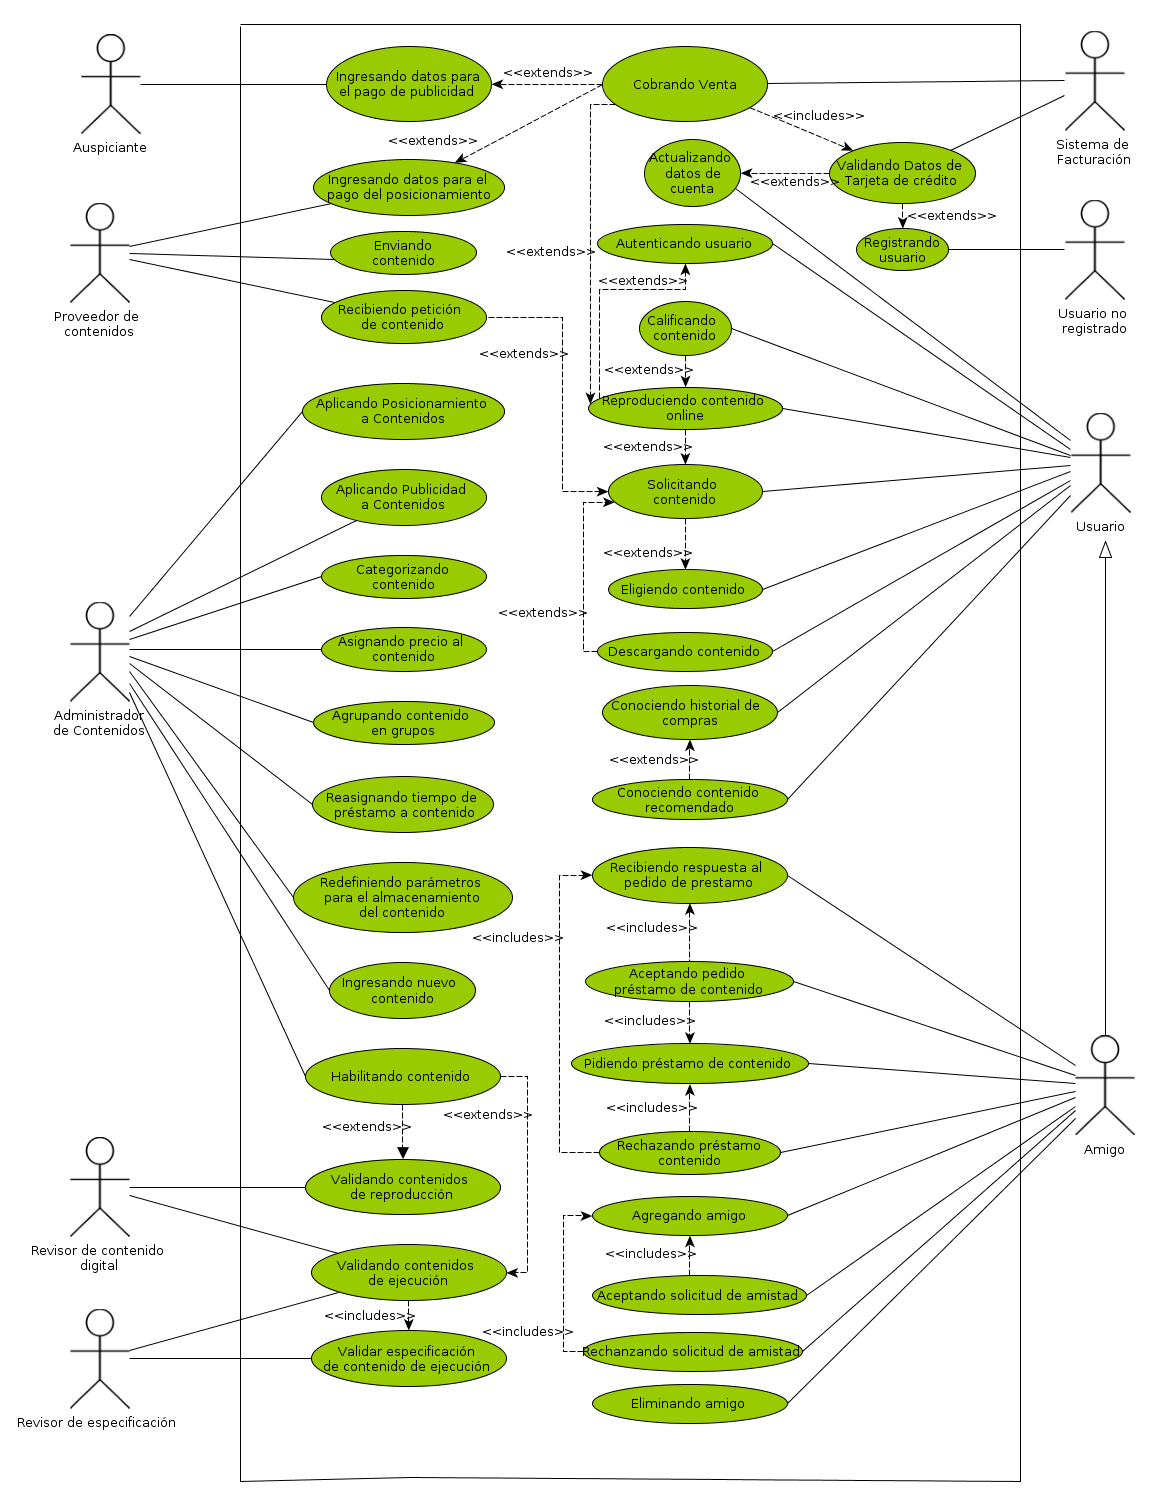
\includegraphics[scale=0.37]{Diagramas/01-CasosdeUsoCU.png}
	\end{center}

\newpage

\subsection{Diagrama de Actividad}

		

	\begin{center}
		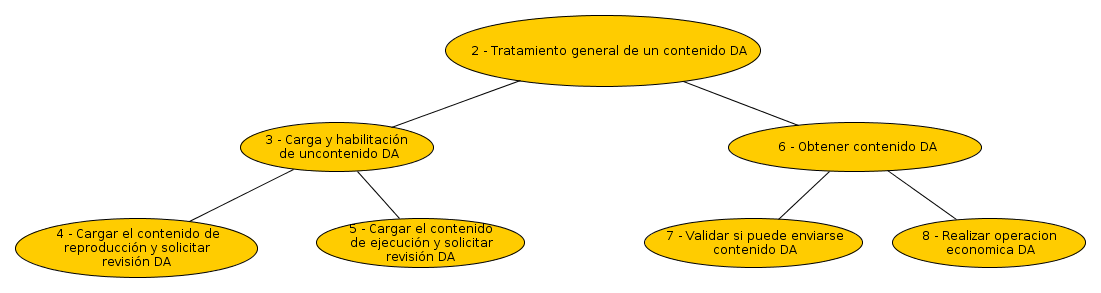
\includegraphics[scale=0.37]{Diagramas/00-DiagramaDeDiagramas.png}
	\end{center}

	\begin{center}
		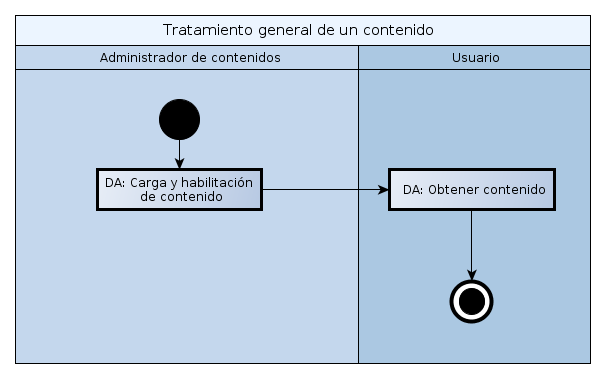
\includegraphics[scale=0.37]{Diagramas/02-TratamientoGeneralDeUnContenidoDA.png}
	\end{center}

	\begin{center}
		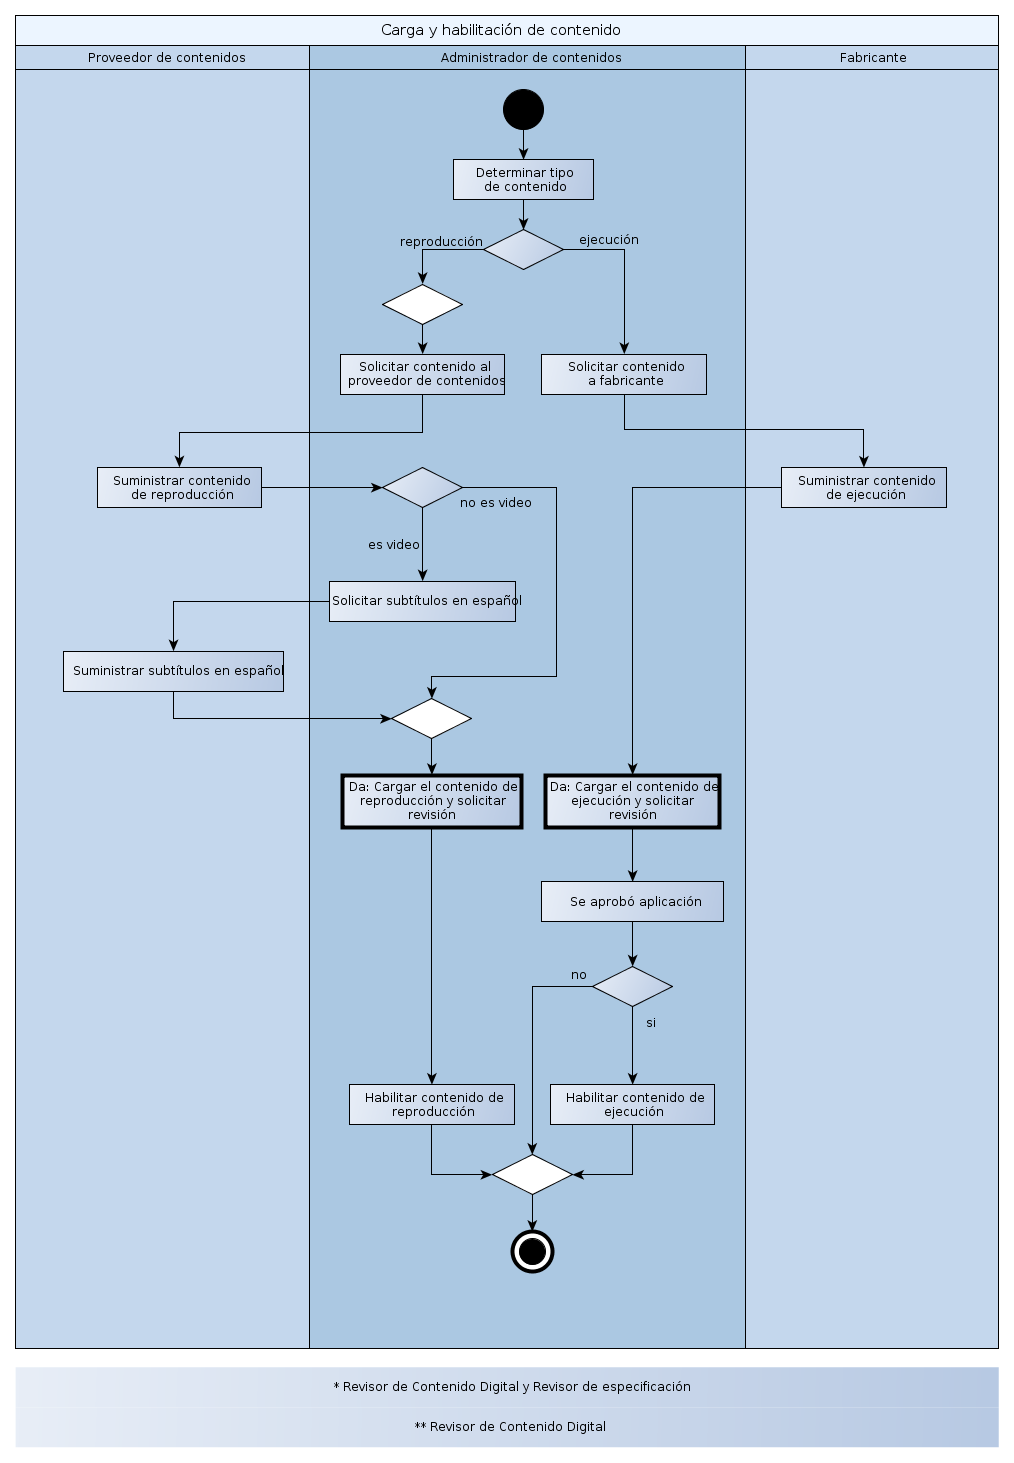
\includegraphics[scale=0.37]{Diagramas/03-CargaYHabilitacionDeContenidoDA.png}
	\end{center}

	\begin{center}
		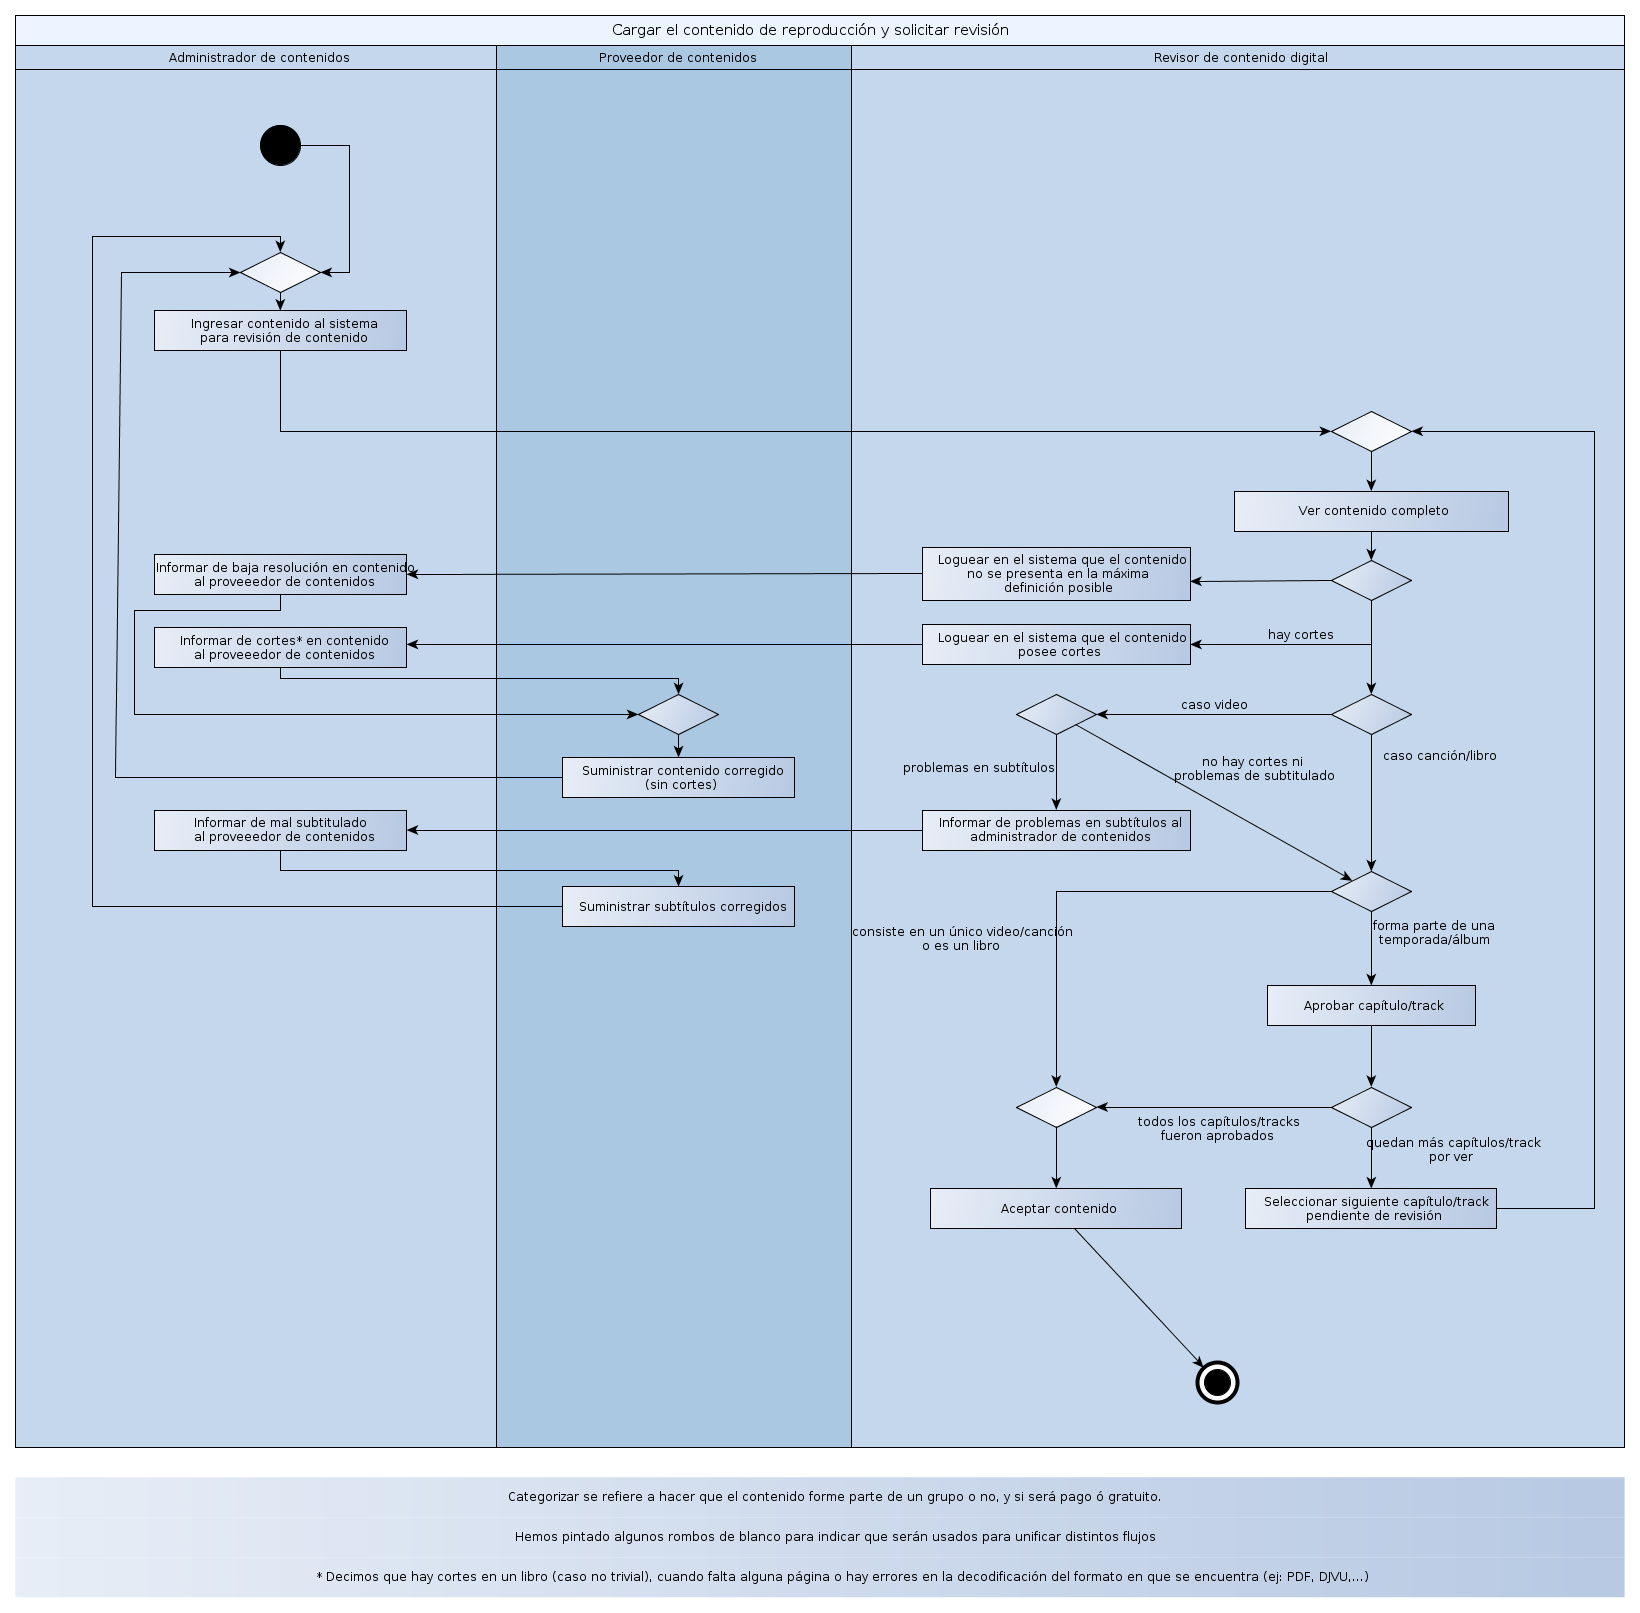
\includegraphics[scale=0.37]{Diagramas/04-CargarElContenidoDeReproduccionYSolicitarRevisionDA.png}
	\end{center}

	\begin{center}
		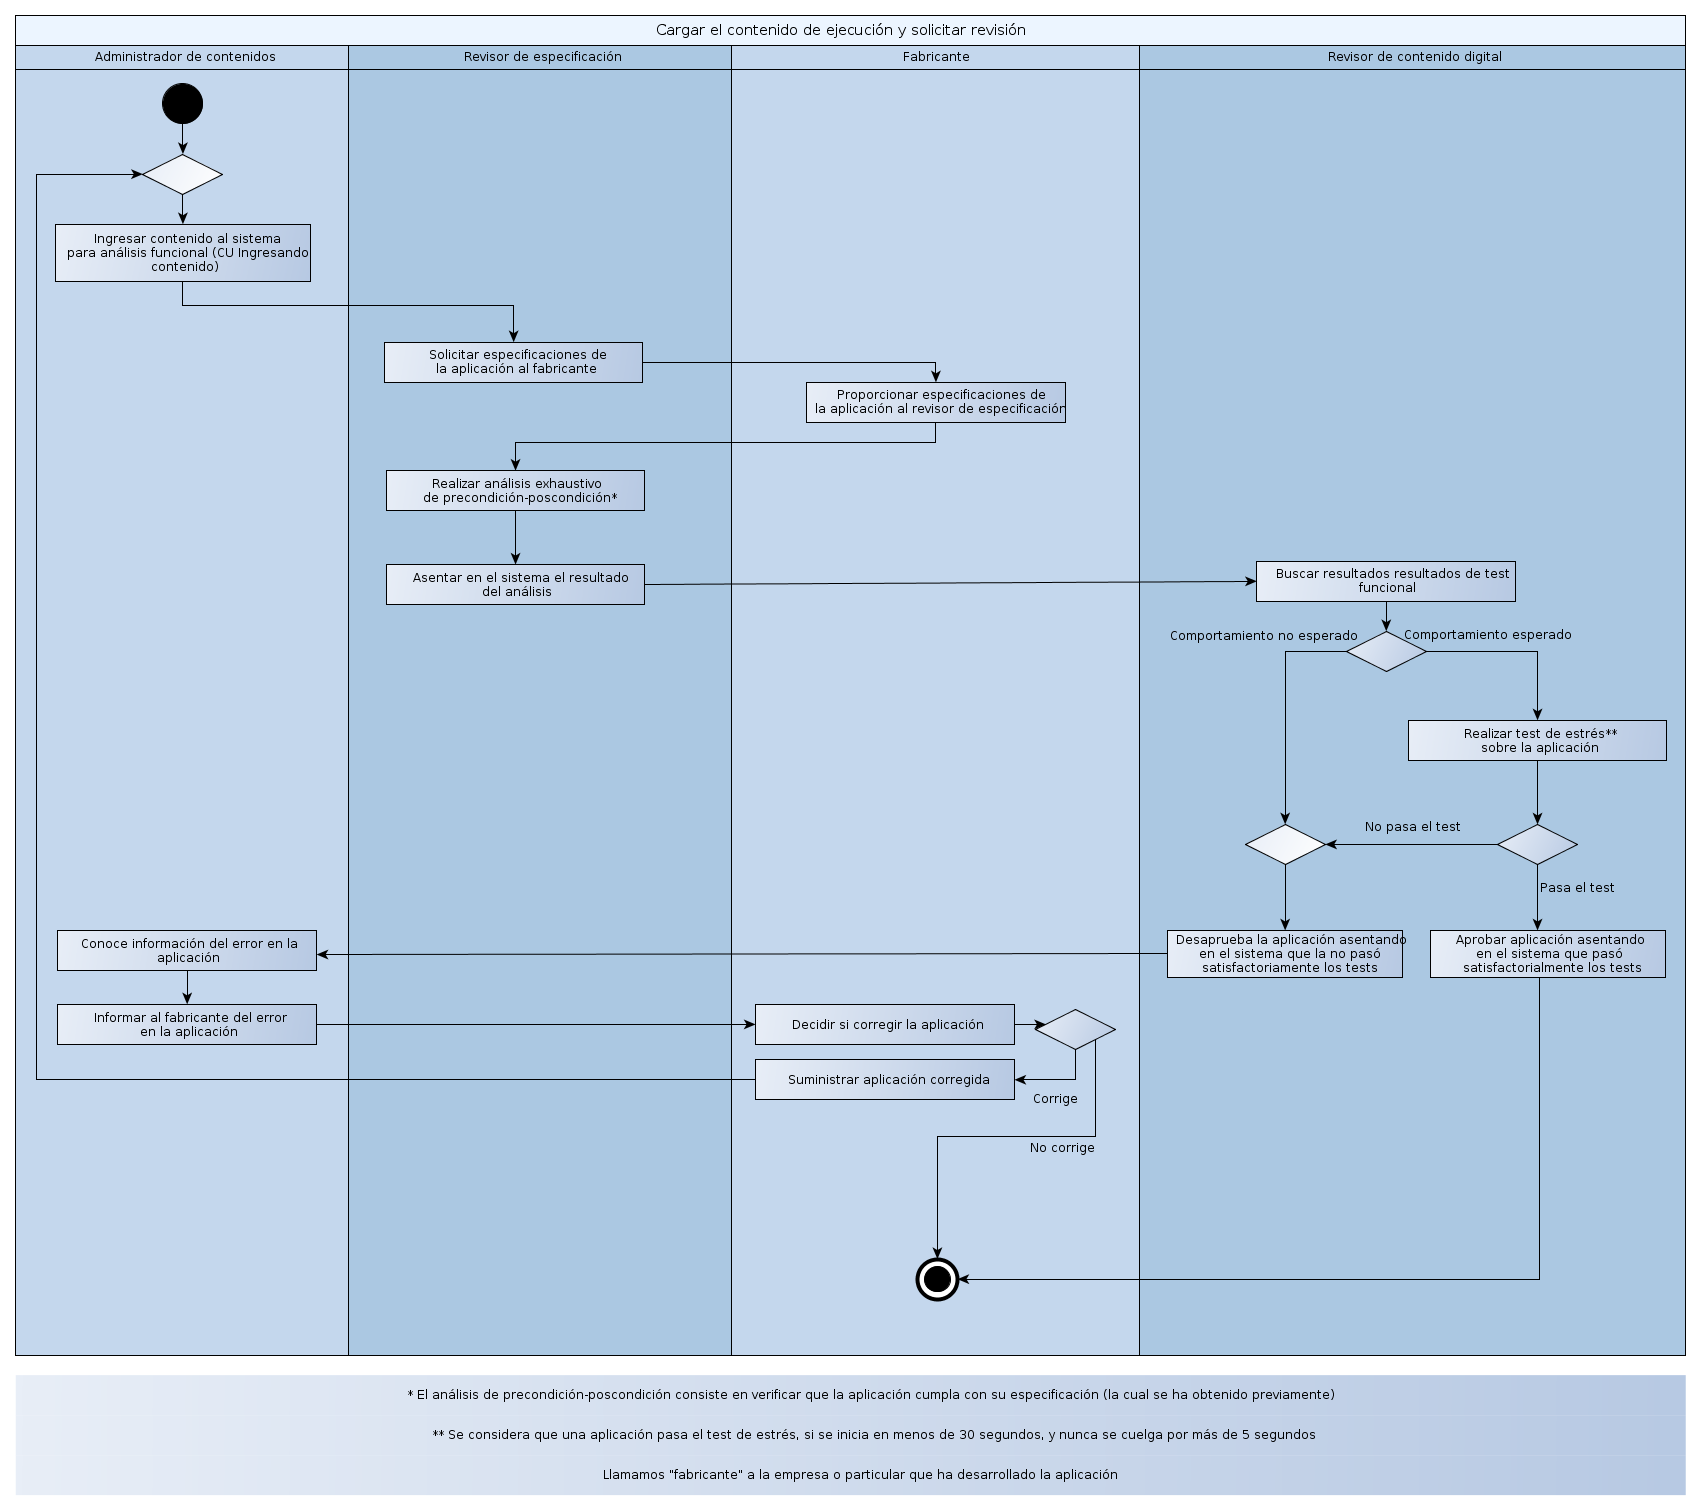
\includegraphics[scale=0.37]{Diagramas/05-CargarElContenidoDeEjecucionYSolicitarRevisionDA.png}
	\end{center}

	\begin{center}
		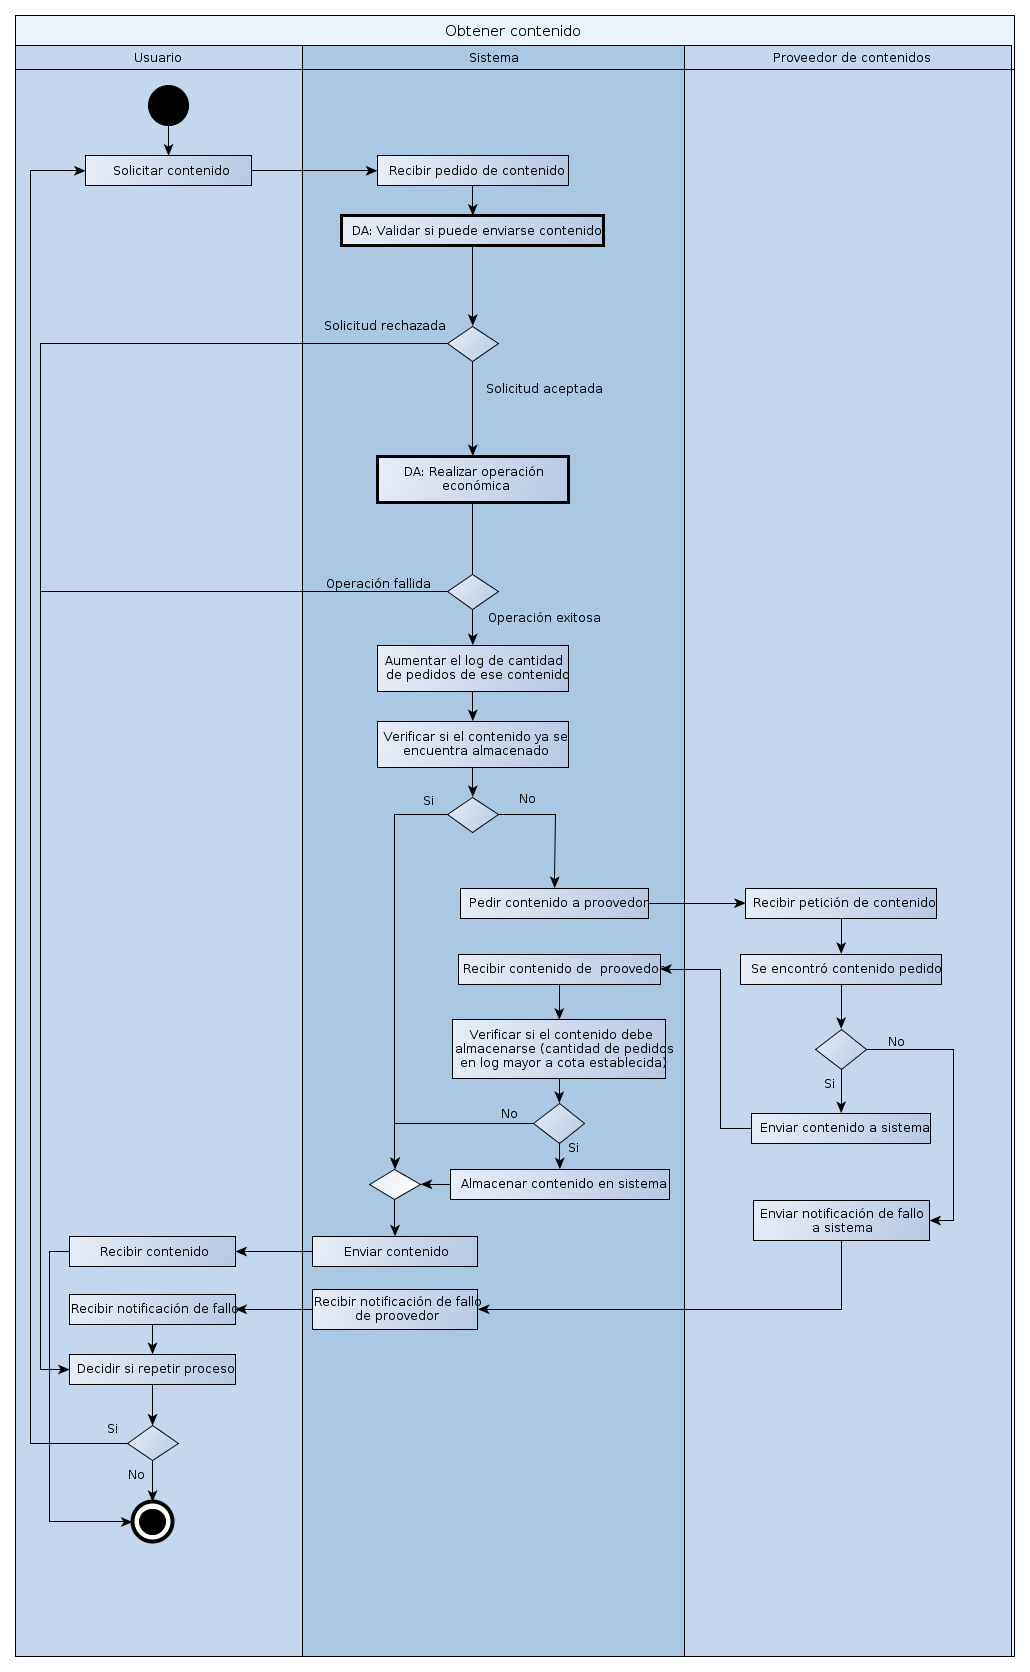
\includegraphics[scale=0.37]{Diagramas/06-ObtenerContenidoDA.png}
	\end{center}

	\begin{center}
		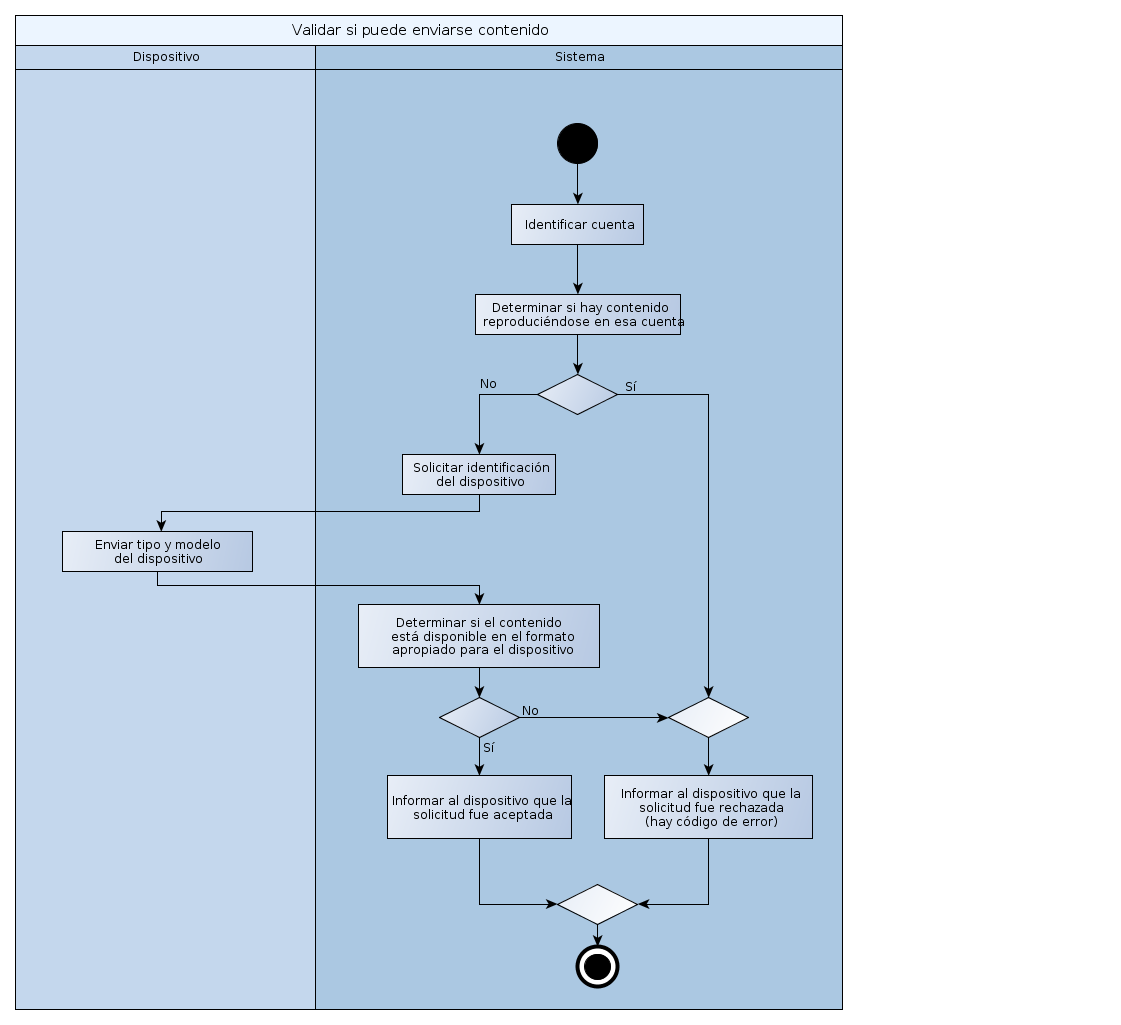
\includegraphics[scale=0.37]{Diagramas/07-ValidarSiPuedeEnviarseContenidoDA.png}
	\end{center}

	\begin{center}
		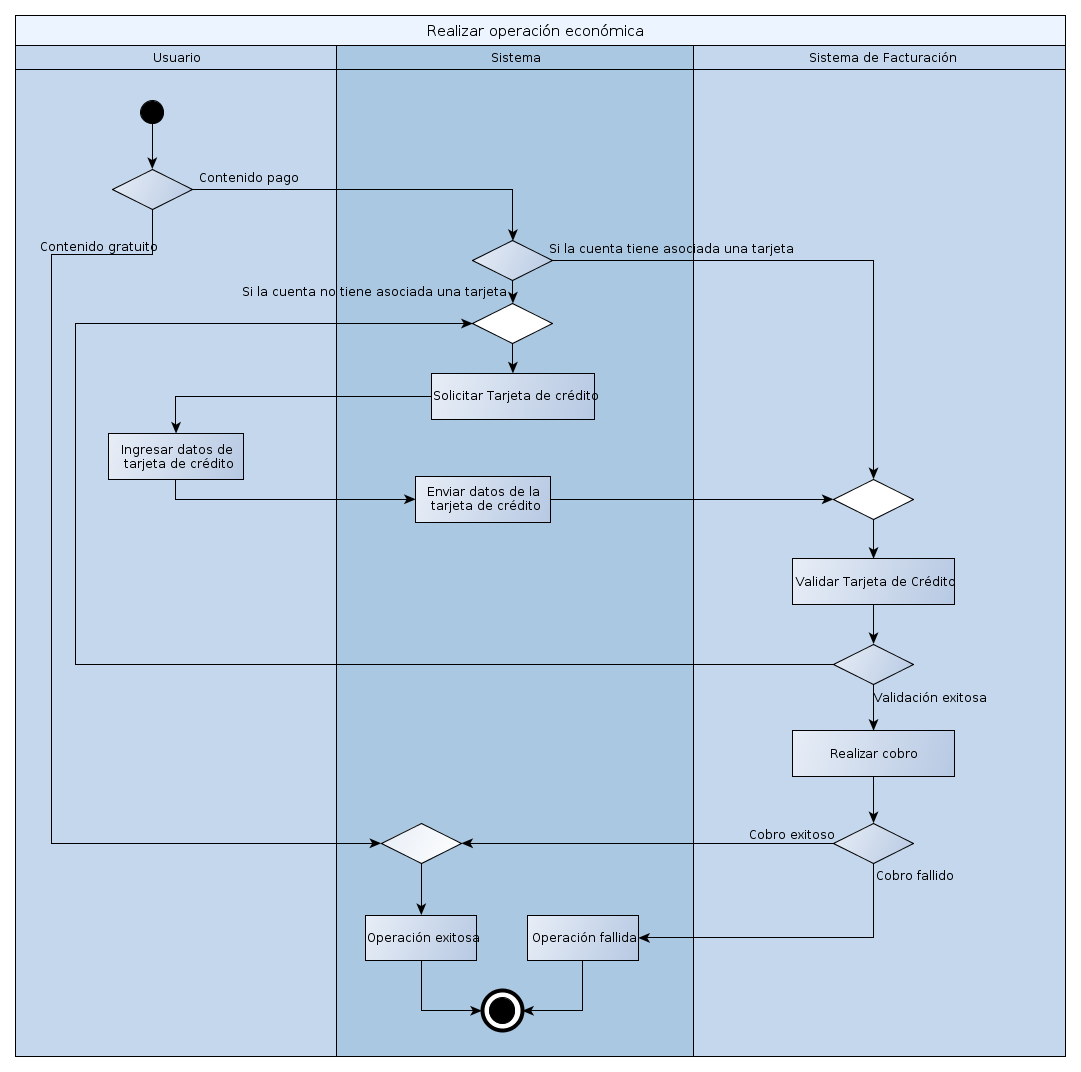
\includegraphics[scale=0.37]{Diagramas/08-RealizarOperacionEconomicaDA.png}
	\end{center}

	\begin{center}
		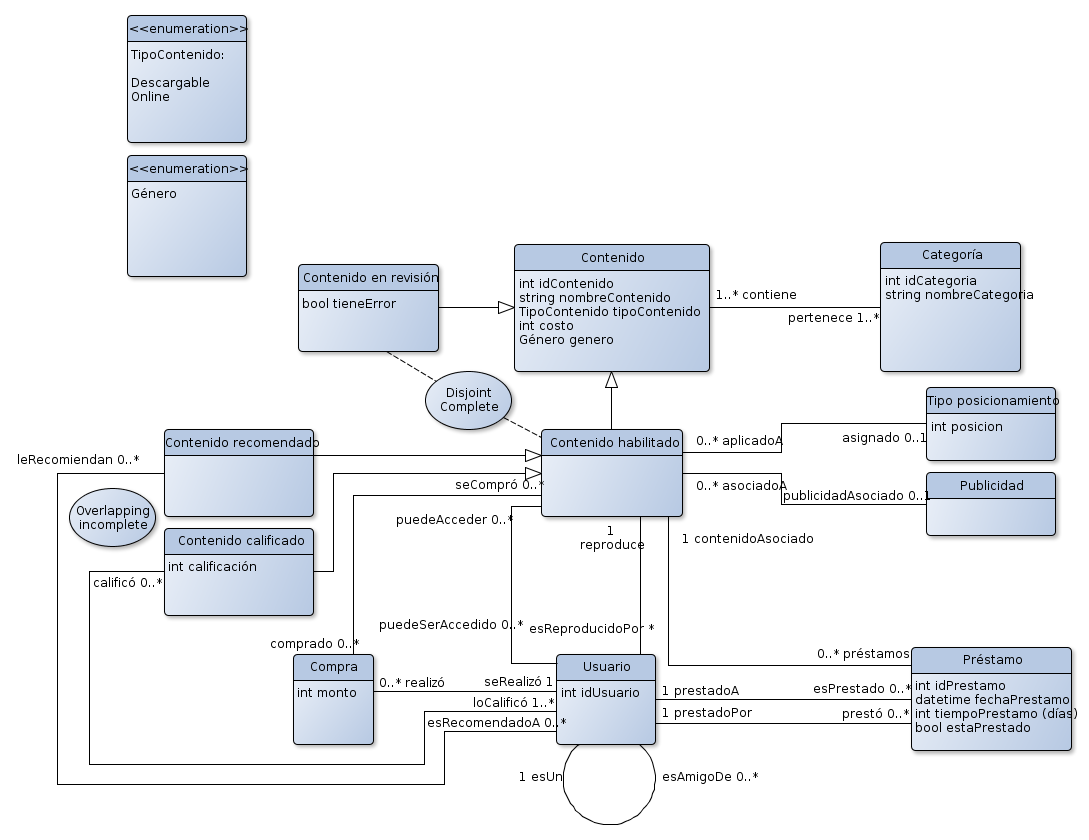
\includegraphics[scale=0.37]{Diagramas/09-ModeloConceptualMC.png}
	\end{center}

\subsection{Modelo Conceptual}


	
\section{Trazabilidad}



\newpage

\end{document}
